\section{Balken}
    \subsection{Formulierungen}
        % 2 Möglichkeiten: Statische und Kinematische Formulierung.\\
        % \textbf{Statische Formulierung:} GGB \& SG erfüllt, KR zum Teil nicht. Generell zu weich.
        % \textbf{Kinematische Formulierung:} GGB \& SG nicht erfüllt, KR schon. Steifer als echt. Schlechte approx mit nur einer Funktion. Approximation wird besser durch besseren Ansatz und mehrere Elemente.
        \subsubsection{Statische Formulierung}
            GGB \& SG erfüllt, KR zum Teil nicht. Generell zu weich.
            \\\textit{Ansatz:} Balkenränder Spannungsfrei ($\sigma_{22}=\sigma_{33}=\tau_{13}=\tau_{23}=0$). $\sigma_{11} \neq 0$ aus $M_z$ und $\tau_{12} \neq 0$ aus $Q_y$.
            \begin{center}
                $\displaystyle\sigma_{11}=-\frac{M_z(x)}{I}\cdot y$
            \end{center}
            \vspace{-3mm}
            \textit{Vorgehen:}
            \vspace{-2mm}
            \begin{itemize}
                \item Beanspruchung am Balken ermitteln (MechII)
                \item Spannungen $\sigma_{11}$ und $\tau_{12}$ aus Beanspruchung berechnen (MechII). (Muss GGB erfüllen)
                \item Dehnung $\varepsilon$ mit SG ermitteln
            \end{itemize}
        \subsubsection{Kinematische Formuliereung}
            GGB \& SG nicht erfüllt, KR schon, muss stetig sein. Steifer als echt. Schlechte approx mit nur einer Funktion. Approximation wird besser durch besseren Ansatz und mehrere Elemente.
            \\\textit{Ansatz:} Verschiebungsfeld $\underline{u}$ auswählen, welches KR erfüllt (Bsp. $u_y(x) = a\cdot x^3+b\cdot x^2$
            \\\textit{Vorgehen:}
            \vspace{-2mm}
            \begin{itemize}
                \item Falls möglich Koeff mit KR bestimmen
                \item Spannungen $\sigma_{ij}$ mit SG bestimmen
                \item Restliche Koeff durch Verfahren von Ritz bestimmen.
            \end{itemize}
            \vspace{1mm}
            
    \subsection{Energiesätze}
        \subsubsection{Definitionen}
            \begin{itemize}
                \item Spannungsfeld $\sigma_{ij}(x,y,z)$ zulässig falls: GGB \& \textit{stat} RB erfüllt.
                \item Verschiebungsfeld $u_i(x,y,z)$ zulässig falls: stetig \& \textit{kin} RB erfüllt (schwächere Bedingung).
                \item Verschiebungsfeld \& Spannungsfeld verträglich iff SG erfüllt.
                \item Deformationsenergie: $U=\frac{1}{2}\iiint_V \sigma_{ij}\cdot\varepsilon_{ij}dV$
                \item Potential äussere Energie:\\
                $V=-\iiint_V f_i\cdot u_idV-\sum_{a}\underline{F}_a\cdot\underline{u}_a$
                \item Potentielle Energie: $E_p=U+V$
                \item Komplementäre Deformationsenergie:\\ $U_K=\iiint_V(\oint_0^{\sigma_{ij}}\varepsilon_{ij}d\sigma_{ij})dV := U$  (lin. elast.)
            \end{itemize}
            
        \subsubsection{Satz vom Minium der potentiellen Energie (SMPE)}
            Aus der Menge der zulässigen \textbf{Verschiebungsfelder} $u_i^*(x,y,z)$ \& der damit verträglichen Spannungsfelder $\sigma_{ij}^*(x,y,z)$ macht das wirkliche Verschiebungsfeld $u_i(x,y,z)$ $E_P$ \textbf{minimal}.
            \[E_p(u_i) < E_p(u_i^*)\]
            %\textit{Direkte Anwendung:} Ansatz für $u_i(x,y,z,a_\gamma)$, zulässig (stetig, KRB erfüllt). Berchene $\varepsilon_{ij}^*$ (aus KR) und verträgliche Spannungen $\sigma_{ij}^*$ (aus SG). $\sigma_{ij}^*$ braucht nicht zulässig zu sein (GGB \& SRB evtl. nicht erfüllt). Berechne $E_p(u_i^*)$ und bestimme $a_\gamma$ mit $\frac{\partial E_p}{\partial a_\gamma}=0$.
            \textit{Direkte Anwendung:}
            \begin{enumerate}
                \item Ansatz für $u_i(x,y,z,a_{\gamma})$
                \item $\varepsilon_{ij}^*$ und $\sigma_{ij}^*$ berechnen (GGB \& SRB evtl. nicht erfüllt)
                \item $E_p$ berechnen
                \item Koeff mit \textbf{Verfahren von Ritz} ermitteln.
                \[\frac{\partial E_p}{\partial a_{\gamma}} =0\]
            \end{enumerate}
            
        \subsubsection{Bsp}
            Ansatz:\\
            $u_y=ax^3+bx^2; \quad u_x=-\frac{du_y}{dx}y= -(3ax^2+2bx)y; \quad u_z = 0$\\
            KR: $\varepsilon_{xx} =(-6ax-2b)y; \quad \varepsilon_{yy}=\varepsilon_{zz}=\varepsilon_{xy}=\varepsilon_{yz} = \varepsilon_{xz}=0$\\
            SG: $\sigma_{xx} = \alpha(-6ax-3b)y; \quad \sigma_{xy}=\sigma_{xz}=\sigma_{yz}=0$\\ $\sigma_{yy}=\sigma_{zz}=2G\frac{\nu}{1-2\nu}(-6ax-2b)y$\\
            SMPE/ \textbf{Verfahren von Ritz:}\\
            $U=\frac{1}{2}\int_0^l\int_\frac{-h}{2}^\frac{h}{2}\int_{-\frac{b}{2}}^\frac{b}{2}(\sigma_{xx}\cdot\varepsilon_{xx})dzdydx=6\cdot\alpha\cdot I\cdot l(\alpha^2l^2+\frac{b^2}{3}+abl)$\\
            $V=-P\cdot u_y(x=l)=-P(al^3+bl^2)$\\
            $E_p=6\alpha Il(a^2l2+\frac{b^2}{3}+abl)-P(al^3+bl^2)$
            %\vspace{-3mm}
            \small\[\frac{\partial E_p}{\partial a} = 0 \Rightarrow a=-\frac{P}{6\alpha I};\quad\frac{\partial E_p}{\partial b} = 0 \Rightarrow b=-\frac{P}{2\alpha I}\]\normalsize
        \vspace{-3mm}    
        
        \subsubsection{Satz vom Min. der kompl. Deform-energie (SMkDE)}
            Aus der Menge der zulässigen \textbf{Spannungsfelder} $\sigma_{ij}^*(x,y,z)$ \& damit verträglichen $\varepsilon_{ij}^*(x,y,z)$ macht das wirkliche Spannungsfeld $\sigma_{ij}(x,y,z)$ die komplementäre Deformationsenergie $U_K$ \textbf{minimal}. 
            \[U_K(\sigma_{ij}) < U_K(\sigma_{ij}^*)\]
            %\textit{Direkte Anwendung:} Ansatz für $\sigma_{ij}^*(x,y,z,a_\gamma)$, zulässig (GGB, SRB erfüllt). Berechne $\varepsilon_{ij}^*$ (aus SG), nicht unbedingt zulässig (KR, KRB eventuell nicht erfüllt). Berechne $U_K(\sigma_{ij}^*)$ und bestimme $a_\gamma$ mit $\frac{\partial U}{\partial a_\gamma}=0$.
            \textit{Direkte Anwendung:}
            \begin{enumerate}
                \item zulässiger Ansatz für $\sigma_{ij}^*(x,y,z,a_{\gamma})$ (GGB \& SRB erfüllt) 
                \item $\varepsilon_{ij}^*$ berechnen (KR evtl. nicht erfüllt)
                \item $U_K(\sigma_{ij}^*)$ berechnen
                \item Koeff mit \textbf{Verfahren von Ritz} ermitteln (siehe oben)
            \end{enumerate}
            
        \subsubsection{SMPE \& FEM}
            \begin{wrapfigure}[5]{r}{0.5\linewidth}
                \vspace{-2mm}
                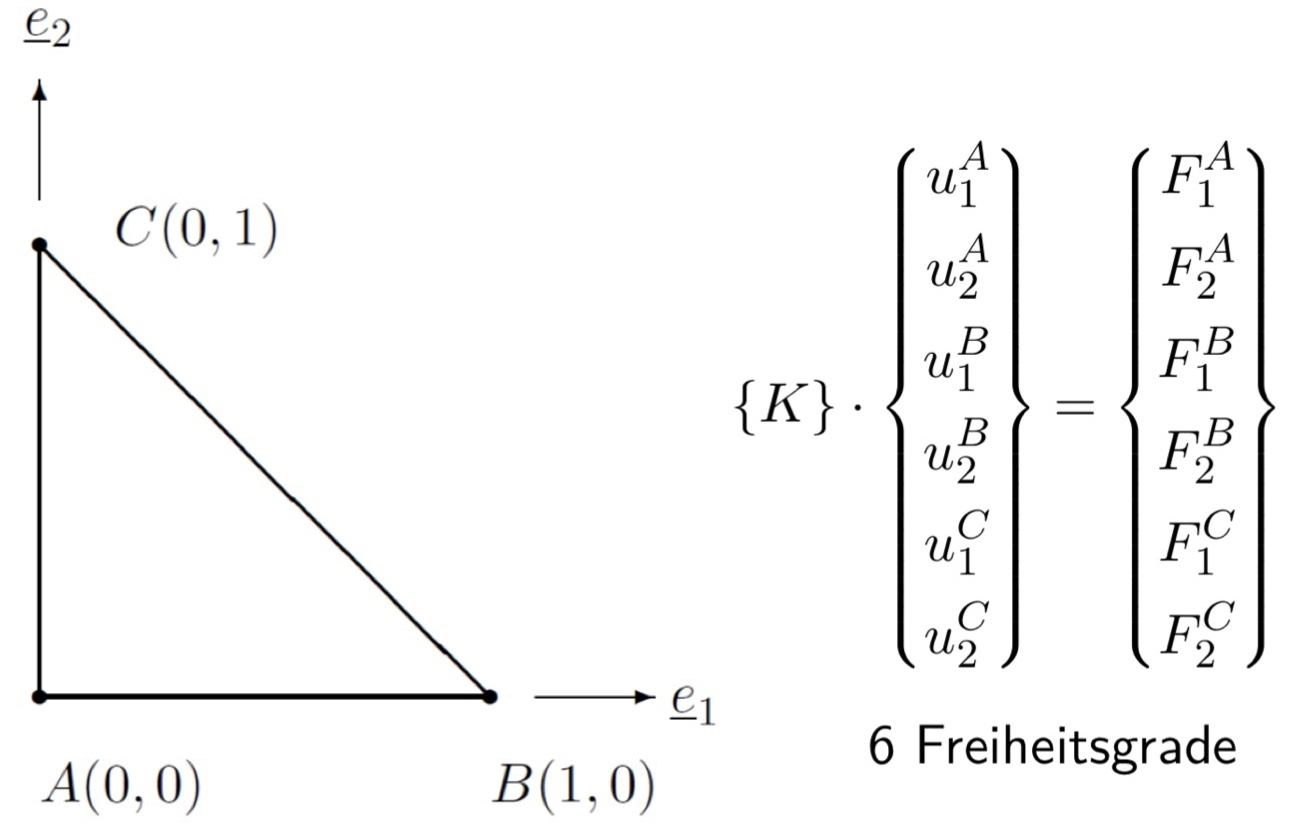
\includegraphics[width=\linewidth, height=25mm]{02/Dreieckselement}
            \end{wrapfigure}
            Relation der Verschiebungsfreiheitsgrade der Knoten ($\{u\}$) und äusseren Kräften an den Knoten ($\{F\}$) über die \textbf{Elementsteifigkeitsmatrix} ($\{K\}\in\mathbb{R}^{6\times6}$): $\{F\}=\{K\}\{u\}$\\\\
            
        \subsubsection{Bsp}
            Ansatz: $u_1=ax_1+bx_2+c$; $u_2=dx_1+ex_2+f$
            %$\Rightarrow u_1(x_1=0,x_2=0)=c=u_1^A$; $\quad u_2(x_1=0,x_2=0)=f=u_2^A$;...\\
            % $\varepsilon_{11}=(u_1^B-u_1^A)$; $\varepsilon_{22}=(u_2^C-u_2^A)$; $\varepsilon_{12}=\frac{1}{2}(u_2^B-u_2^A+u_1^C-u_1^A)$
            \begin{itemize}
                \item Koeff aus RB: $\Rightarrow u_1=(u_1^B-u_1^A)x_1+(u_1^C-u_1^A)x_2+u_1^A$; $u_2=\dots$
                \item $\varepsilon_{ij}((u_1^A,...,u_2^C)$, $\sigma_ij(u_1^A,...,u_2^C,E,\nu)$ bestimmen
                \item $U=\frac{1}{2}\frac{1}{2}(\sigma_{11}\cdot\varepsilon_{11}+\sigma_{22}\cdot\varepsilon_{22}+2\sigma_{12}\cdot\varepsilon_{12})\cdot t$ mit Dicke $t$ und Fläche $\frac{1}{2}$.
                \item $V=-(F_1^A\cdot u_1^A+F_2^A\cdot u_2^A+...+F_2^C\cdot u_2^C)$
                \item $E_p=U+V=E_p(u_1^A,...,u_2^C,E,\nu,t)=\alpha_1(u_1^A)^2+\alpha_2u_1^Au_1^B+ ...-(F_1^Au_1^A+...)$
                \item Minimum $E_p:$ $\displaystyle\frac{\partial E_p}{\partial u_i^\kappa}=0$ mit $i=1,2$ \& $\kappa=A,B,C$ (6Gl)
                \item Bsp: $\displaystyle\frac{\partial E_p}{\partial u_1^A}=0 \Leftrightarrow \frac{\partial U}{\partial u_1^A}=-\frac{\partial V}{\partial u_1^A}$ (lin. Fkt. in $u_1^A,..,u_2^C$) 
                \item $\Rightarrow F_1=\kappa_{11}u_1^A+...+\kappa_{16}u_2^c$; $\kappa_{11},...,\kappa_{16}$: 1. Zeile von $\{K\}$
            \end{itemize}
            